\documentclass{assignment}
\usepackage{graphicx}
\begin{document}

\assignmentTitle{Mykola Vaskevych}{22372199}{assets/images.jpg}{Foundations of Computer Science 2}{Homework Exercises 2}

\section*{Section A}
Static type checking occurs during code compilation when the compiler determines whether the types of variables and expressions used in the code are compatible. 
Here are all the moments where type-checking occurs in the code:
\begin{enumerate}
    \item Variable declaration: The compiler checks the types of the variables being declared, for example:\hword{char x='a';}

    \item Operator usage: When we use the "+" operator to concatenate two strings, or for arithmetic operations, for example: \hword{s1+ " "+ s2+ " " + s3}

    \item Variable assignment: When variables are assigned to each other, the compiler checks that the types are compatible, for example: \hword{x=y;}.

    \item Method calls: The compiler checks that the arguments passed to methods match the expected parameter types, for example: \hword{System.out.println(Arrays.toString(myArray1));}.

    \item Object instantiation: The compiler checks that the type of the object being instantiated matches the class being used, for example: \hword{Random r1 = new Random(5);}.

    \item Conditional statements: The compiler checks that the expression in a conditional statement is a boolean, for example: \hword{(s1==s2?"t":"f")}.

In general, type checking occurs whenever a type is used in a way that the compiler needs to ensure it is consistent and appropriate.

Below, near each moment when type checking occurs, I have written a comment with marks as to why it happens there. The comet will be of the following type: \hword{//due to points (1) and (3)}
\end{enumerate}



\section*{Code}
\lstinputlisting[language=Java]{assets/code.java}

\section*{Section B}
When a variable is assigned to another variable, a copy of the value or the object's reference is made. For example, on line "x = y" the value of "y" is copied to "x", and any following changes to "y" will not affect "x". In the line, "myArray2 = myArray3", the reference of "myArray3" is copied to "myArray2", and any next changes made to "myArray2" will not affect "myArray3".

For objects, meaning variables contain a reference to the same object in memory. When an object is assigned to another variable, the reference to the object is copied but not to the object itself. For example, in the line, "s3 = new String("xyz")", a new String object is created in memory, and the reference to it is assigned to "s3", but "s1" and "s2" still referencing the old String object, so any changes made to the new String object will not affect the old String object.

The impact of these different semantics on memory is that copy semantics creates copies of values or references, meaning each variable points to a separate piece of memory. On the other hand, reference semantics mean that variables share the same object in memory, which can lead to unexpected behavior if changes to one variable affect the object shared among all variables.

When the line s2 = "abc" is executed, for instance, a new String object is created, and s2 is given access to it. As a result, any modifications that will be made to s2 will not change the previous String object, and s1 and s3 will continue to refer to it. Nevertheless, when the line s1 = s2 is executed, the reference to the new String object is copied to s1, meaning that s1 now corresponds to the same object in memory as s2.

\section*{Section C}
Garbage collection occurs when an object is no longer accessible through any reference variable. In this code, garbage collection occurs whenever a reference variable previously pointed to an object is assigned a new value or is no longer in use.

Specifically, garbage collection occurs on the following lines:
\begin{itemize}
    \item x=y:\hword{"a"} previously referenced by "x".

    \item myArray2=myArray3: the original array previously referenced by myArray2 \hword{"\{'f','g','h','i','j'\}"}.

    \item r2=r1: the original Random object \hword{"new Random(5)"} previously referenced by r2 .

    \item s2="abc": the String object previously referenced by s2 \hword{"xyz"}.

    \item s1=s2: the String object previously referenced by s1 \hword{"abc"} .

    \item s3=new String("xyz"): the String object previously referenced by s3 \hword{"abc"}.
\end{itemize}


\textbf{All highlighted things the garbage collector will delete from the memory heap.}






\newpage
\section*{Section D}
\begin{figure}[h]
    \centering
    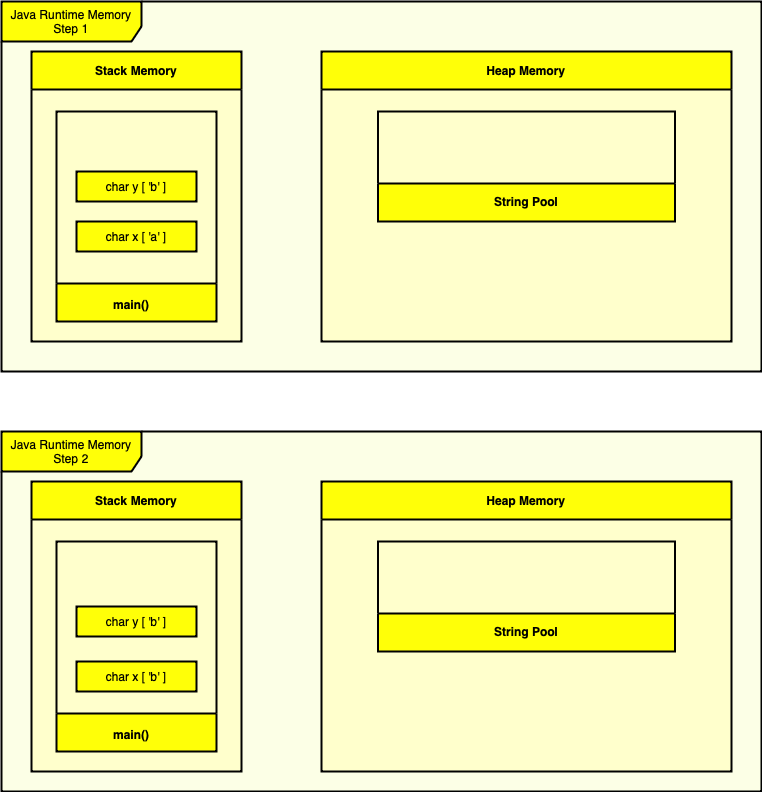
\includegraphics[scale=0.6]{assets/homework2diagram(1-2).png}
    \caption{Step 1 and 2}
\end{figure}
\begin{figure}[p]
    \centering
    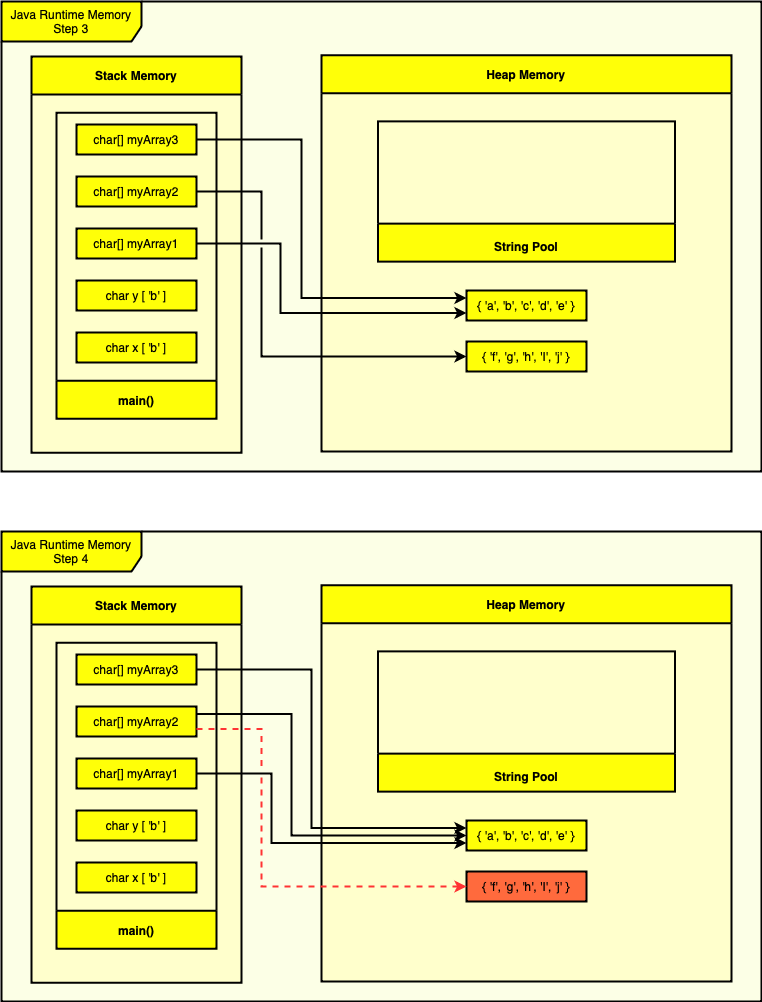
\includegraphics[scale=0.6]{assets/homework2Diagram(3-4).png}
    \caption{Step 3 and 4}
\end{figure}
\begin{figure}[p]
    \centering
    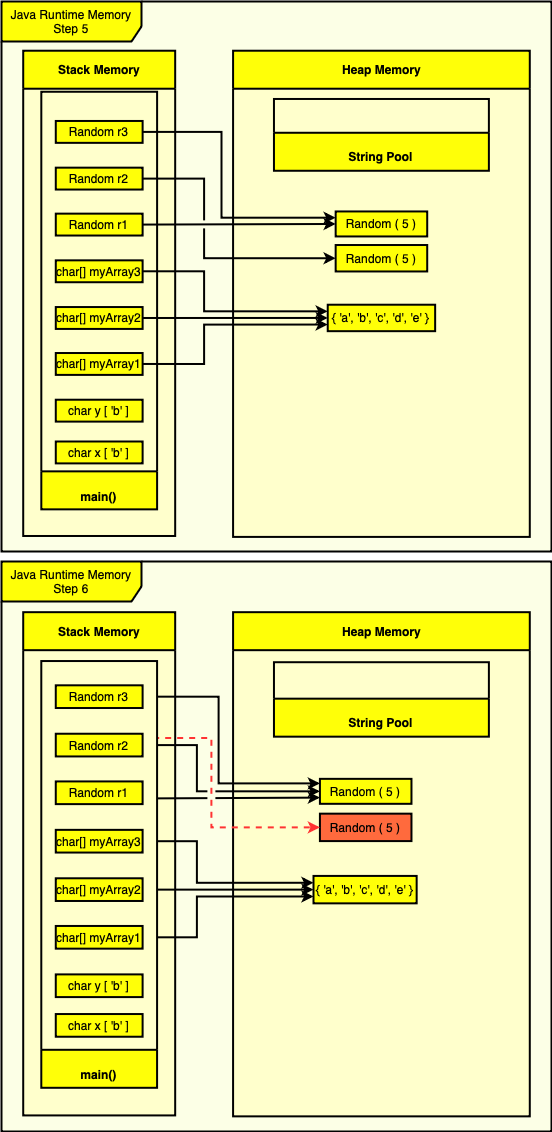
\includegraphics[scale=0.55]{assets/homework2Diagram(5-6).png}
    \caption{Step 5 and 6}
\end{figure}
\begin{figure}[p]
    \centering
    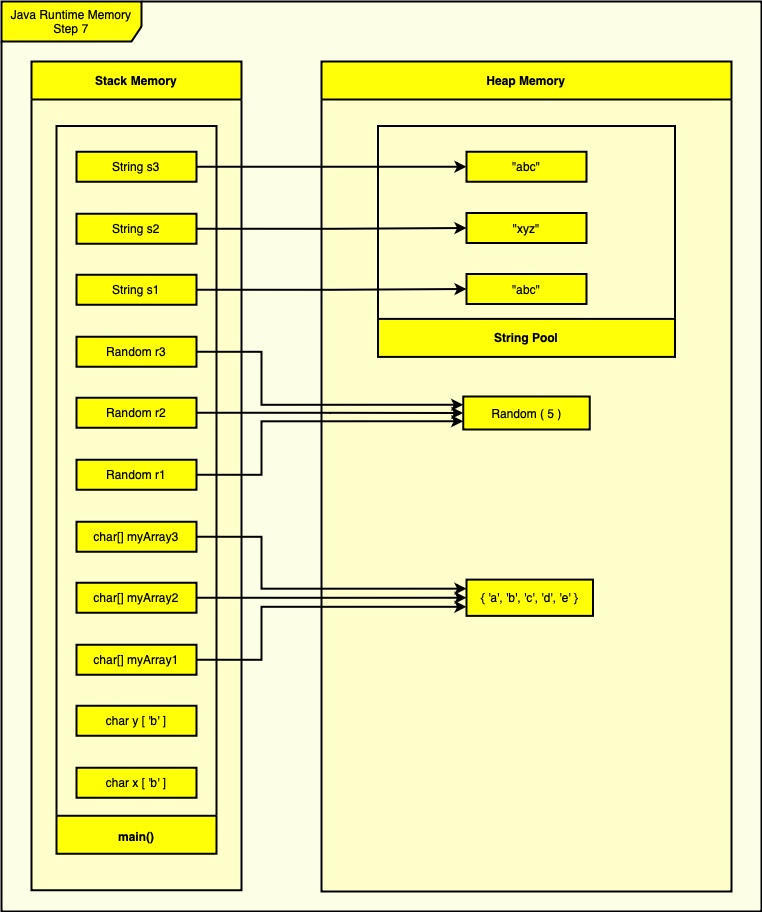
\includegraphics[scale=0.6]{assets/homework2Diagram(7).png}
    \caption{Step 7}
\end{figure}
\begin{figure}[p]
    \centering
    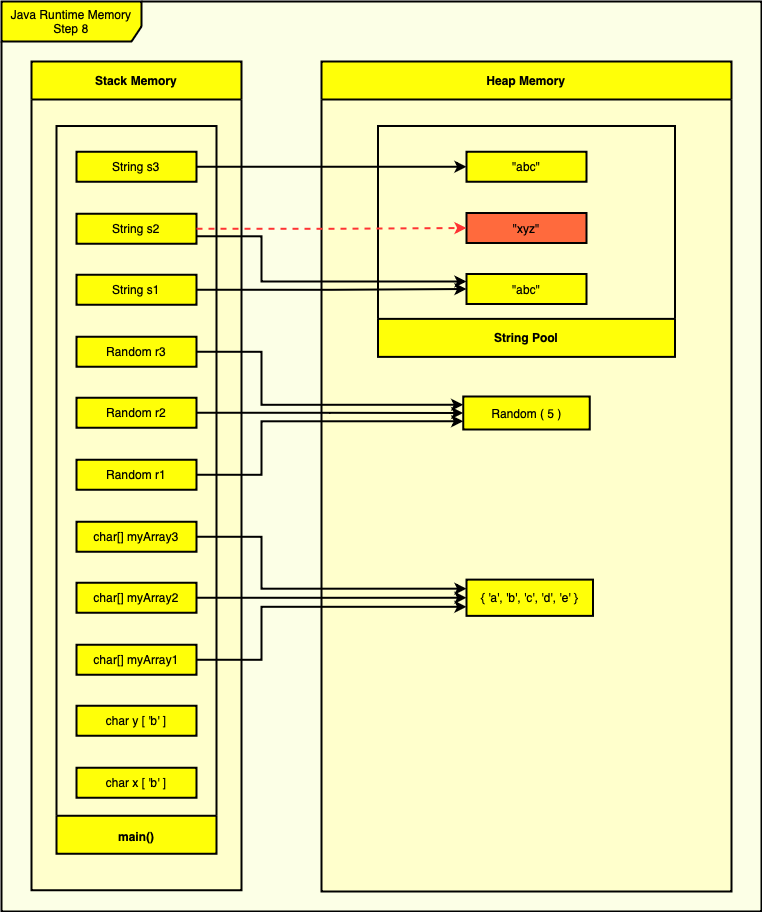
\includegraphics[scale=0.6]{assets/homework2Diagram(8).png}
    \caption{Step 8}
\end{figure}
\begin{figure}[p]
    \centering
    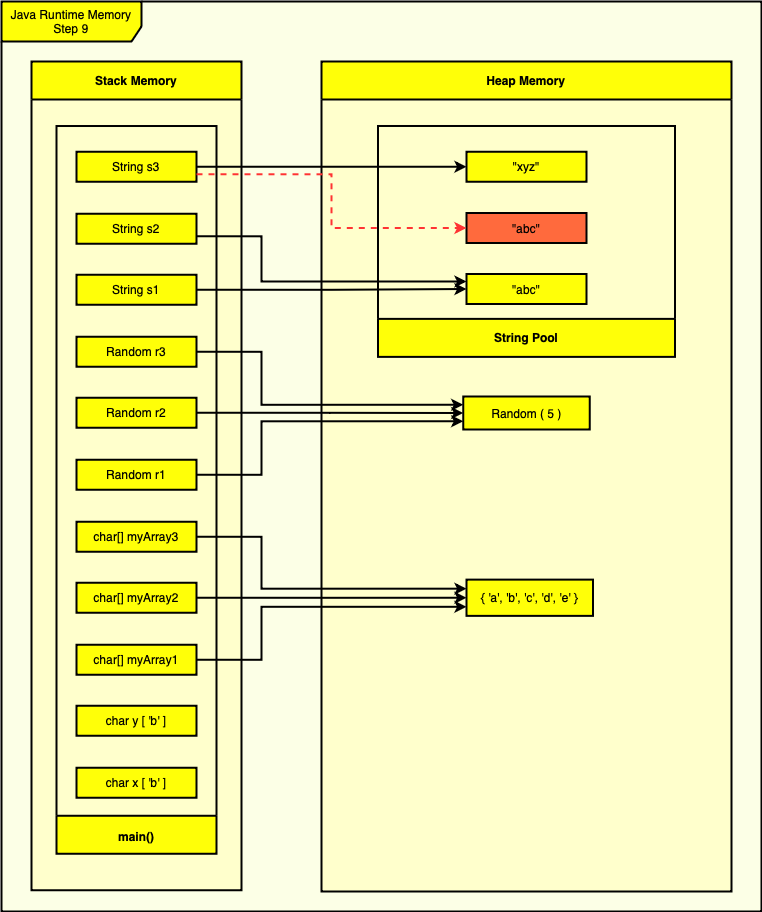
\includegraphics[scale=0.6]{assets/homework2Diagram(9).png}
    \caption{Step 9}
\end{figure}


\newpage
\section*{Section E}
\lstinputlisting[language=Java]{assets/output.java}

\end{document}
